
\begin{figure}[ht]
\centering

\begin{subfigure}[b]{0.55\textwidth}
    \centering
    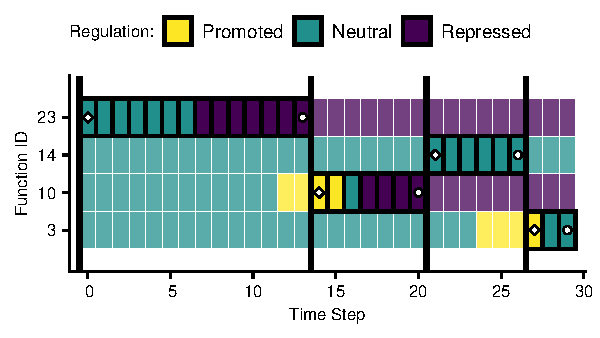
\includegraphics[width=\linewidth]{chapters/05-tag-based-genetic-regulation/media/signal-counting-networks/case-study-trace-id-20203-regulator-state-horizontal.pdf}
    \caption{\small Module regulation over time.}
    \label{chapter:tag-based-regulation:subfig:rst-exec-trace}
\end{subfigure}%
\hfill
\begin{subfigure}[b]{0.3\textwidth}
    \centering
    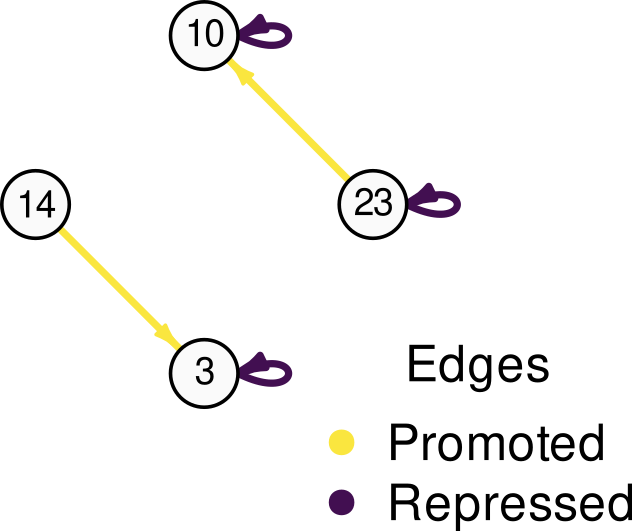
\includegraphics[width=\linewidth]{chapters/05-tag-based-genetic-regulation/media/signal-counting-networks/case-study-id-20203-network.png}
    \caption{\small Regulatory network.}
    \label{chapter:tag-based-regulation:subfig:rst-reg-network}
\end{subfigure}%


\caption{\small 
   \textbf{Execution trace of a SignalGP program solving the four-signal version of the signal-counting task.}
    Color denotes each function's regulatory state (yellow: promoted, purple: repressed) during evaluation; functions not regulated or executed are omitted.
    Functions that are actively executing are annotated with a black outline.
    Black vertical lines denote input signals, and a diamond (white with black outline) indicates which function was triggered by the input signal.
    A circle (white with black outline) indicates which function executed a response.
    (b) shows the directed graph representing the regulatory network associated with trace (a).
    Vertices depict functions that either ran during evaluation or were regulated. 
    Each directed edge shows a regulatory relationship between two functions where the edge's source acted on (promoted in yellow or repressed in purple) the edge's destination.
    Note that in the case presented here all repressing relationships are self-referential.
    }
    
\label{chapter:tag-based-regulation:fig:signal-counting-example-networks}
\end{figure}
